To try and gain an in depth understanding of the Ethereum blockchain and Solidity, I chose to implement the popular game Texas Hold'Em Poker \cite{texasHoldEm}. Due to time limitations, the difficulty of the project, and previous experience with front-end technologies, I chose to not implement a front-end for the game and to instead spend my time learning Solidity.

The flow gameplay of Texas Hold'Em is depicted in Figure 1.

\begin{wrapfigure}{r}{0.3\textwidth}
	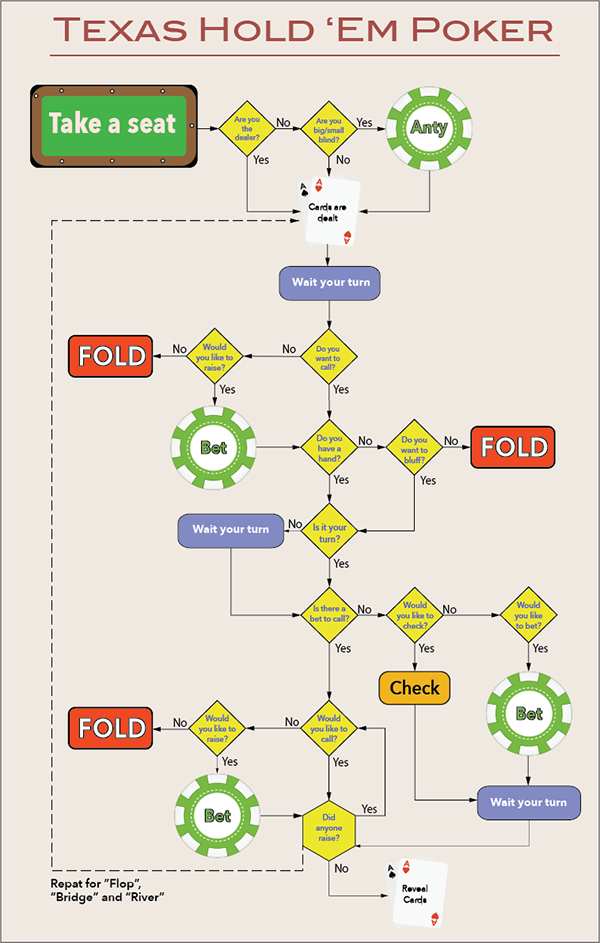
\includegraphics[width=0.3\textwidth]{flow}
	\caption{The gameplay flow of Texas Hold'Em Poker}
	\label{fig:key}
\end{wrapfigure}

When there are at least two players at the table the game may be started. The player to the left of the dealer pays the small blind, and the player to the left of him plays the big blind (two required monetary deposits to ensure there is some risk every round). The cards are then dealt, and betting ensues. When every player has either met the maximum bet, or folded (sacrificing their current stake in the game), some number of cards are placed on the table. At first three cards are played (called the "flop"), then one card is added (called the "turn"), then a final card is added (called the "river"). The flop, turn, and river cards are only played once each round of betting has concluded. After the river is played, there is a final round of betting, after which all players cards are revealed and the pot (the communal sum of bets) is distributed to the winner(s).

There has been a lot of interest in implementing gambling games, including poker, on the blockchain. The decentralised nature of the blockchain removes the need for trust to be placed on the casino. The casino is responsible for storing all players hands, storing all players bets, performing correct game logic, and for paying the winners. In one case, online casino website Absolute Poker went bankrupt \cite{abspoker}, leaving players currently owed by the casino with no payouts. By implementing the application on the blockchain, there is the potential to remove the requirement for trust in all of these features \cite{trust}.